\section{Le POSIX 1003.1}

%regarder bien le passer

Traditionnellement les système qui implémentions les patron POSIX avaient une système simple et puissante de permission, quand même, certain problèmes ont arrive, et éventuellement les problèmes ont apparaître. 

Après savoir la nécessite de régler sur le domaine de sécurise et non seulement les ACL, une groupe a était forme pendant la définition de la famille de patron POSIX 1003.1. Les premières documents POSIX qui ont été considère ces question étaient les document 1003.1e (\emph{System Application Programming Interface}) et 1003.2c (\emph{Shell and Utilities}), cependant, la première approximation de ce sujet était trop ambitieuse. Les groupe responsable pour le patronisation avait centre ces effort dans une tas assez grande de choses, lesquelles  comprenant \emph{Access Control Lists} (ACL), \emph{Audit}, \emph{Capability},\emph{ Mandatory Access Control }(MAC), et \emph{Information Labeling}\cite{aclsuse}.

En Janvier de 1998\cite{aclsuse} le financement était fini, par contre, le travaille n'était pas prés. De toute façon le dixsèptieme brouillon a été publique quand même\cite{posix17}.

Donc après cette an, les système UNIX appelé "\emph{trusted}" (Trusted Solaris, Trusted Irix, Trusted AIX ont été développer avec quelque parts de la documentation 17. Ces systèmes ne sont pas complètement compatible entre eux. 

Aujourd'hui la plupart des système UNIX et UNIX-like support ACL. Ces implémentassions sont usuellement compatible avec le document 17. Le projet TrustedBSD aussi avait ajouter les ACL sur les système BSD. Les ACL e les MAC  FreeBSD-RELEASE avaient apparu en 2003.

Les base des ACL sont lancé sur le système traditionnel présent usuellement dans presque tous les système UNIX, alors, avant de préciser sur les ACL on parlerais du modelé traditionnel.

\subsection*{Système de permission Traditionnel}

%Les groups e les permission
Le modelé traditionnel POSIX offre trois group de utilisateur qui sont le propriétaire, le group e les autres. Chaque group a une octet que indique les permission de lecture (\textbf{r}ead), écrire (\textbf{w}rite) et exécution (e\textbf{x}ecute). La première classe fournit les permission pour le utilisateur que rempli le rôle de propriétaire, ensuite, vient les droits pour le groupe principal du propriétaire enfin les droites pour touts les autres utilisateurs. 
 
%Explication simple
Après les trois octets peut venir le \emph{Set User Id}, \emph{Set Group Id} et \emph{Sticky bit}, lesquelles sont utilisé dans certain cases. Il faut faire attention avec le \emph{Sticky Bit}, il permit les utilisateur normale d'exécuter les utilitaire comment le administrateur(\emph{root}), par contre, quelque manque de sécurité peut compromettre le système entière.

%Le droit du root
Seulement le \emph{root} peut créer les groups e changer les association de groupes. Celui-là que aussi peut changer les propriétaire. 

\subsection*{Les ACL}

%Basic Definitions
Dans une modèle de de sécurise ACL, si quelque agent faire une requête pour accéder aux donnés, il faut consulte les ACL pour une entrée que permettre l'opération demandé. Chaque ACL est une ensemble de règles d'accès. Les règles possible peut-être regarder dans le tableau ci-dessous(\ref{entree}).
\begin{center}
\begin{tabular}{|l|l|}
  \hline
    \multicolumn{2}{|c|}{Les types de ACL} \\
  \hline
	\textbf{Type d'entrée} & \textbf{format} \\
  \hline
	Propriétaire & user::rwx \\
	Utilisateur nommée & user:name:rwx  \\
	Groupe propriétaire & group::rwx \\
	Groupe nommée & group:name:rwx \\
	Masque & mask::rwx \\
	Autres & other::rwx \\   
  \hline
\end{tabular}
\label{tab:entree}
\end{center}

Le format des règles sont formée par une indicateur de classe (comme les classe du système Traditionnel), une quantificateur pour spécifier de quel utilisateur ou group on parle et les octet de permission.

%EXPLIQUER MELLEIUR
Avec cette représentation le sens de la classe du groupe a redéfini comment le limite supérieur de les permission de chaque entrée dans la classe du groupe. Ça arrive parce que les entrée du groupe et du utilisateur nommées seront désigner à entrée du groupe. Aussi, c'est importante rappeler que cette choix permettre se prémunir contre les application qui ne sont pas conscient de les ACL.
\footnote{Fabricio: Je ne comprend pas cette affirmation, je laisse ici le teste orignial: 
These named group and named user entries are assigned to the group class, which already contains the owning group entry. Different from the POSIX.1 permission model, the group class may now contain ACL entries with different permission sets, so the group class permissions alone are no longer sufficient to represent all the detailed permissions of all ACL entries it contains. Therefore, the meaning of the group class permissions is redefined: under their new semantics, they represent an upper bound of the permissions that any entry in the group class will grant. This upper bound property ensures that POSIX.1 applications that are unaware of ACLs will not suddenly and unexpectedly start to grant additional permissions once ACLs are supported.}.

Les ACL qui sont équivalent avec le mode simple de permission de fichier s'appellent minimale et ils ont trois entrée. Si les ACL peut avoir plusieurs entrée ont les appelle étendu. Tous les ACL étendu doivent avoir l'entrée masque et peut contenir théoriquement n'importe combien de entrée. On verrais après que ce numéro d'entrée peut-être limitée pour chaque implémentassions et que aussi il est important pour la performance.

%EXPLIQUER MELLEIUR
Dans les ACL minimale les permission de classe groupe sont égale à les permission de groupe propriétaire, cependant, dans les ACL étendu on peut avoir les entrée avec plusieurs utilisateurs et/ou groupes, quelques de cette entrées peut-être contenir permissions qui la classe groupe n'aurais pas, alors, on peut avoir une inconsistance basée en le cas qui les permissions du groupe propriétaire sont diffèrent de les permission de la classe groupe. 

On résoudre ce problème avec le masque. Comme on peut observer dans le figure (\ref{fig:img_acl-mapping}), il y a deux cas: les permission de la classe groupe seront déguise pour la masque tandis que les permission de l'entrée du groupe propriétaire encore définit les permission pour le groupe propriétaire.    


\begin{figure}[htbp]
	\centering
		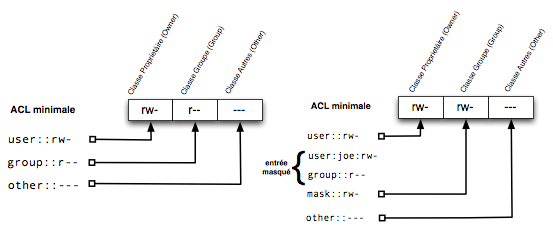
\includegraphics[height=3in]{img/acl-mapping.jpg}
	\caption{caption}
	\label{fig:img_acl-mapping}
\end{figure}


Pour assurer le consistance, quand une application change les permission (par exemple le commande \emph{chmod}) les ACL sont modifiée de façon a reproduire ce modification. 

On a dit que le permission de la classe groupe sont calculée comme le limite supérieur de tous les entrée dans le classe group. Avec les ACLs minimaux cette computation est simple, par contre, avec les ACLs étendu, on a besoin de masquer les permissions. Comme l'exemple de le tableau (\ref{tab:masquee}), les entrée de permission qui sont partie de la classe de groupe et qui aussi sont présente dans l'entrée masque sont applique effectivement. Si une permission était absent dans le masque, c'est a dire que aucun entrée de group (qui non le groupe du propriétaire) peut avoir ce permission, on dit dans ce cas qui la entrée est masquée.  

\begin{center}
\begin{tabular}{|l|l|l|}
  \hline
    \multicolumn{3}{|c|}{La masque de permissionL} \\
  \hline
	\textbf{Type} & \textbf{Format} & \textbf{Permission} \\
  \hline
	Utilisateur nommée & user:jean:r-x  & r-x\\
  \hline
	Masque & mask::rw- & rw-\\
  \hline
	\multicolumn{2}{|c|}{Permission Effective} & r--\\
  \hline
\end{tabular}
\label{tab:masque}
\end{center}

\subsection*{Algorithme de vérification}

Pour vérifier les droits d'accès de une objet du système de fichier il y a une algorithme assez simple.\footnote{Il faut traduire cette algorithme lá :-)}

%changer le titre et la langue
\begin{algorithm}
\caption{Vérifie se une utilisateur peut ou ne peut pas accéder une objet du système de fichier}
\label{algacl}
\begin{algorithmic}
\IF{the user ID of the process is the owner}
	\STATE the owner entry determines access
\ELSIF{the user ID of the process matches the qualifier in one of the named user entries}
	\STATE this entry determines access 
\ELSIF{one of the group IDs of the process matches the owning group and the owning group entry contains the requested permissions} 
	\STATE this entry determines access
\ELSIF{one of the group IDs of the process matches the qualifier of one of the named group entries and this entry contains the requested permissions}
	\STATE this entry determines access
 
\ELSIF{one of the group IDs of the process matches the owning group or any of the named group entries, but neither the owning group entry nor any of the matching named group entries contains the requested permissions} 
\STATE this determines that access is denied

\ELSE
	\STATE the other entry determines access.
\ENDIF
 

\IF{the matching entry resulting from this selection is the owner or other entry and it contains the requested permissions}
	\STATE access is granted 
\ELSIF{the matching entry is a named user, owning group, or named group entry and this entry contains the requested permissions and the mask entry also contains the requested permissions (or there is no mask entry)}
	\STATE access is granted
 
\ELSE
	\STATE access is denied.
\ENDIF
\end{algorithmic}
\end{algorithm}


\subsection*{Héritage mécanisme}

Le patron POSIX règle non seulement sur les accès des objet du système, mais aussi sur le mécanisme de Héritage. Les ACL sont partage en deux type, les \emph{access ACL} (que on a vu jusqu'á maintenant) et les \emph{default ACL} qui comprendre les règles de héritage.  

Quand on parle de l'héritage on parle de les droits qui sont attribue aux objet du système pendand le moment en que il sont crée. Il y une seul type de objet qui peut être associe avec les \emph{default ACL}; les répertoire. Il faut dire que il n'y a aucune sens en donne \emph{default ACL } pour les fichiers, alors que, aucune objet du système peut être crée dans une fichier, aussi, il faut rappeler que les \emph{Default ACL} n'ont pas aucune implication sur les \emph{access ACL}.

Si une répertoire est crée dans une autre, si le première répertoire a \emph{default ACL}, d'accord avec le mécanisme de héritage,  le deuxième aurais le même ACL qui le première (\emph{default} et \emph{access}). Les objets qui ne sont pas répertoire, devons hérite les \emph{access ACL} seulement. 

Chaque \emph{system call} que crée les objets du système de fichier a une \emph{mode parameter}. Ce paramètre peut contenir neuve octet de permission pour chaque classe (propriétaire, groupe et les autres). Les permission effective de chaque objet crée est l'intersection de les permission défini pour les \emph{default ACL} et les spécification dans le \emph{mode parameter}.

Le système traditionnel a une commande pour designer les modes de permission par défaut pour les nouveau fichiers et répertoires: le commande \emph{umask}. Quand il n'y a aucune \emph{default ACL}, le permission effective est détermine par le paramètre de mode moins les permission configuré avec umask. 
